\documentclass[../Proposal.tex]{subfiles}

\begin{document}
\label{sec:lit}


%Relevance to other work:

%seeking correlates of syllabic organization in the phonetic signal,


The question of how evidence for the relatively abstract concept of a syllable can be found in a continuous phonetic signal is relatively old. 
Looking at the timing relations between the onset and the rhyme can show underlying mental representation of syllables.
% How does this stability thing work?
\paragraph{Global vs. local timing}
Phonotactics of languages differ in how syllables can be constructed and what kinds of clusters are allowed where in the syllable. Complex syllable onsets such as /ksl/ may be a valid onset in a language but not in another, while two languages where this onset is valid still differ in their temporal organization of those consonants with respect to the nucleus vowel of the syllable. There have been found two different kinds of consonantal onset organization: \\
\hspace{2cm}\enquote{Global timing refers
to the coordination of a sequence of consonants as a unit with respect to the vowels on
either side. Alternatively, ‘local timing’ refers
to the coordination of a single consonant gesture in a sequence with respect to a neighboring vocalic gesture. It has been hypothesized
by \cite[]{browman1988some} that both
local and global timing play a role in coordinating consonant sequences with adjacent
vowels.} \cite[286]{byrd1995c}\\

\begin{figure}
    \centering
    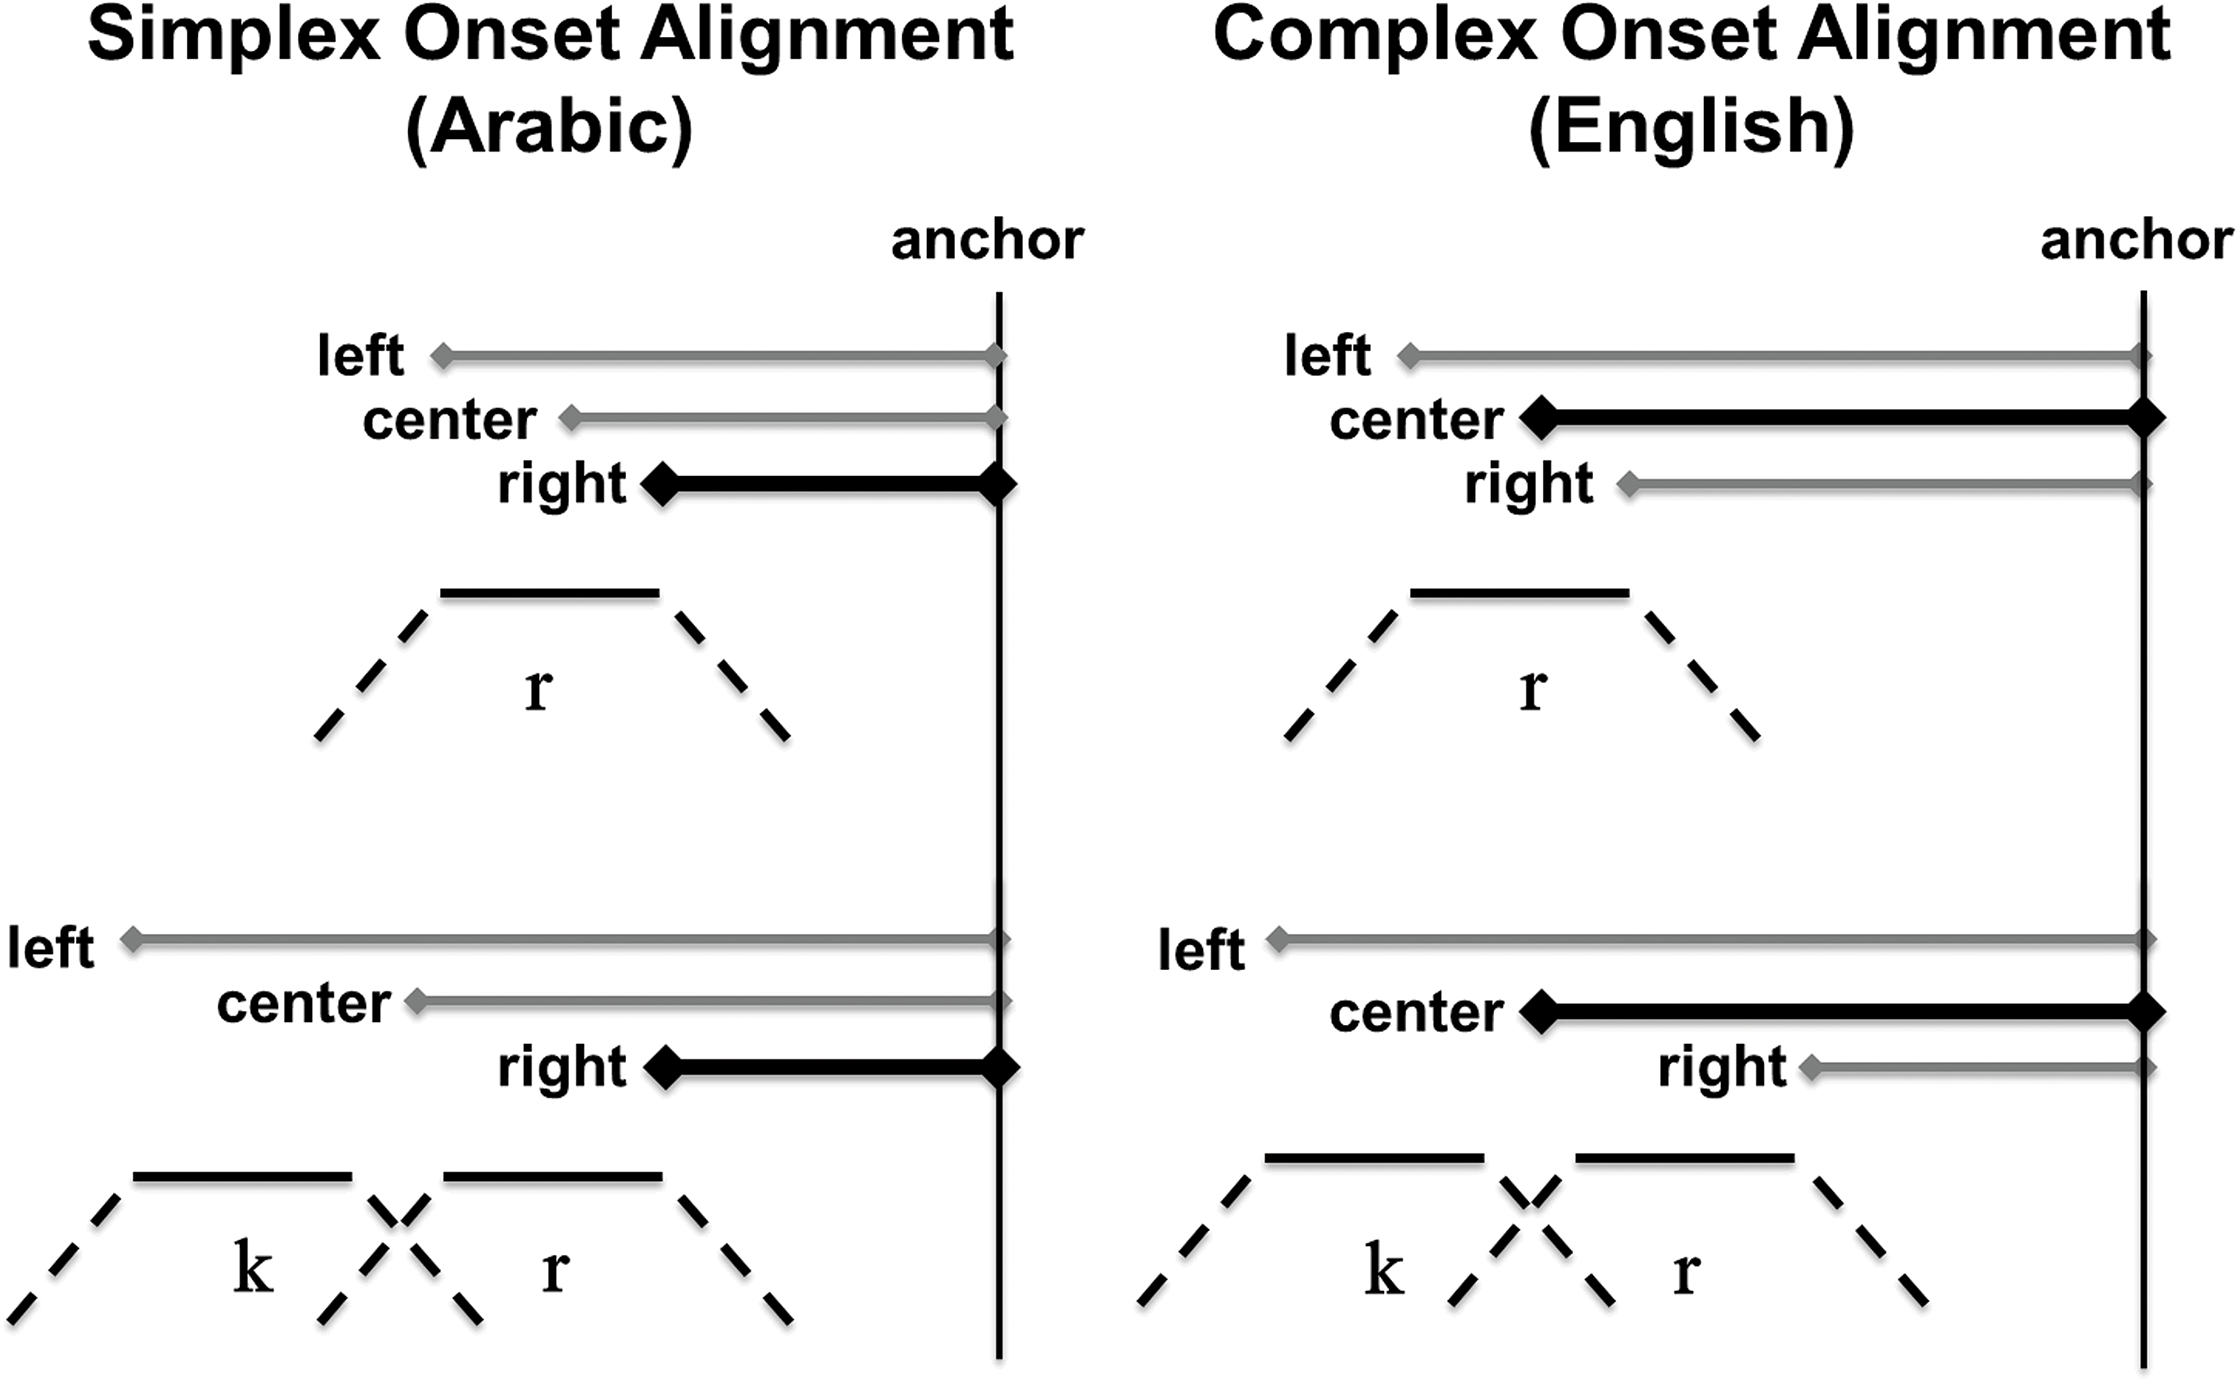
\includegraphics[width=10cm]{figures/onset_alignment.png}
    \caption{Local (Arabic) and global (English) consonant cluster organization: prototypes for simple and CC-cluster onsets showing the respective interval stabilities. From \cite{shaw2015stochastic}, CC BY 4.0.}
    \label{fig:onset_alignment}
\end{figure}

A tool to determine which organization underlies the syllable of a language is the notion of stability. Depending on whether syllable onsets are organized locally or globally, the duration of intervals between the relevant landmarks and a (post-)vocalic anchor varies more or less when more consonants are added to an onset cluster. Landmarks found to be relevant are the right edge (i.e. the offset of the last consonant before the vowel) as for example in Arabic (\cite{shaw2015stochastic}) and the c-center the midpoint between the target and the release of the syllable onset as for example in English (\cite{shaw2015stochastic}). Global timing relates to c-center stability and local timing to stability of the right edge to anchor interval. This stability measure can give a good hint at how syllables in languages are organized, but it is not always sufficient. The concept is illustrated in \cref{fig:onset_alignment} (\cite{shaw2015stochastic}). Besides the stability metric  \cite[]{sotiropoulou2020global} finds other, more nuanced parameters which will be discussed below.

% How does it work for Spanish?
\paragraph{Spanish} \cite{gibson2019temporal} looked at CCVC-syllables in Spanish, at their VOT, gestural plateau duration and gesture overlap. Concerning stability they found patterns that seemed to imply that Spanish does not allow complex syllable onsets (robust IPI) as Arabic does, which organizes consonant clusters locally. 
But, as opposed to Arabic, Spanish has been found to apply overall global timing by \citeauthor{}{sotiropoulou2020global}. In their paper \cite{sotiropoulou2020global} they found that the stability measure is not a reliable tool to detect the underlying syllable organization of Spanish.  Other factors such as voicedness, and manner of articulation can play into the temporal organization of the tongue movements. For instance, the interval stabilities seemed to be quite variable; in voiced stop-lateral clusters, local timing interval stability was found and global timing interval stability in the other instances. So, only a stability metric is not enough to determine a general rule for a language, this is evidence "that syllable structure does not have consistent phonetic manifestations in the articulatory record." \cite[22]{sotiropoulou2020global}.
For sake of the simplicity of this paper, I will nonetheless focus on only stability and the influence of stress while being aware of potentially contradicting results.
% What do we know about stress (in Spanish and the effect it can have on syllables?)?
\paragraph{Stress} In general, according to \cite{prieto2018prosody}, Spanish has a lexical stress / word stress. This can be demonstrated in minimal pairs - or even minimal triples such as in example \ref{ex:stress}. Here, stress is represented by capitalization.

\ex. TERmino - term, end\\
terMIno - finish.\textsc{1sg.prs}\\
termiNO - finish.\textsc{3sg.ipfv}
\label{ex:stress}

These stressed syllables are marked acoustically by \enquote*{longer durations, higher fundamental frequency and higher intensity than unstressed syllables} \cite[215]{prieto2018prosody} although the overall pitch can vary depend on the position of the word in the whole phrase or sentence. \\
There have not been yet studies on the effect of stress in the temporary organization and articulation of Spanish syllables, but results from other languages and the influence of stress on articulation could give us a hint. For instance, in English it has been found by \cite{dejong1993interplay} that coarticulation is reduced in English stressed syllables and locally the articulation is shifted towards the hyperarticulate end of the continuum. A potential pitfall is that that while they ``define stress as the set of prosodic categories which involve relationships of relative prominence between syllables.''\cite[199]{dejong1993interplay} they look at nuclear accent on the whole phrase level in their analysis, which is not exactly what I will be doing (see \cref{sec:methods}). So while intergestural timing is sensitive to the position of the gesture within the prosodic structure of the utterance the influence of stress at the word level is not completely clear.

%%%%% HYPOTHESES %%%%%% 
\paragraph{Hypotheses} 
We know that stress probably will positively influence the timing of syllables since carefully articulated gestures are also longer in duration. I still suppose that the ratio of segment length to intergestural timing will remain the same, i.e. stress will not have an influence on the temporal syllable organization.

\end{document}
%\cite{sotiropoulou2020global}

% words beginning with /pl, bl, kl, gl, pr, kr, tr/ vs. nur /l, r/
% vowel contexts: /a, e, o/
% there is global organization in those clusters:
%     shortening of initial sonorant when in cluster
%     for C-/l/-clusters: reorganization of relative timing of internal CV subsequence
%     early vowel initiation
%     strong compensatory relation between length of open transition (CC) and lateral duration
% simultaneously expressed over a set of phonetic parameters rather than a privileged metric i.e. c-center stability

% Analysis:
%     - interplateau interval IPI (lag between release of C1 and target of C2) in ms (and normalized by length of total constriction duration)
%     - relation between IPI and C2 in CCV -> how duration of C2 responds to changes of IPI
%     - stability analysis: RSD 
%     - Consonant-vowel timing: timing between C2 release (NOFFS) and MAXC of V
%     - vowel initiation

% Results:
%     - the longer the IPI, the shorter the lateral
%     - lateral is shorter if C1 is -voice than when C1 +voice
%     - stability: 
%         - interval stabilities seem to be quite variable
%         - how to: fit linear mixed model with interval duration as DV (log transformated to approximate norm dist), fixed effects: C1, cluster size, voicing, vowel, speaker
%         - vowels do not play a role
%         - for plblgl: C1 voicing affects the way intervals change as the number of consonants increases 
%             - -voice: global timing interval stability
%             - +voice: local timing interval stability
%         - for prbrgr:
%             - global timing interval stability across speakers \& all anchors

%     failure to find consistent results, conclusion: evidence "that syllable structure does not hae consostent phonetic manifestations in the articulatory record." (p22) -> other phonetic consequences (and they then propose those consequences)


% \cite[]{shaw2015stochastic}
% fit the data to different models to achieve a good/perfect fit. I will no attempt this, instead we will stay with descriptive methods.

%would like to read: https://books.google.de/books?hl=de&lr=&id=gDiqDQqO2hwC&oi=fnd&pg=PA273&dq=phonetic+effects+of+stress&ots=m3xQMzgZ0V&sig=D5aTjDDWuFG5f4jGWwG7GHix7-U&redir_esc=y#v=onepage&q=phonetic%20effects%20of%20stress&f=false


% Stress in Spanish: 

% - lexical stress/ word stress 
% - nouns ending in consonant typically have final stress
% - ``lexically-stressed syllables have been reported to have clear acoustic correlates, namely longer durations, higher fundamental frequency and higher intensity than unstressed syllables'' (p.215)
% - pitch: position of the target word in a phrase/sentence will play a role in pitch level
% - duration: mainly dependent on the phrasal level of prominence that  stressed syllables articulation
% - nuclear stress/main phrasal stress normally last content word of sentence, unless a word is emphatically/contrastively in focus

% - see pamies bertrßan 1993 for acoustic correlates of spanish


% - English: reduced coarticulation within stressed sylls
% - One possible description of the difference between more and less stressed syllables is the “sonority expansion” hypothesis, that the jaw is lower in stressed syllables so that more energy can radiate from the mouth.
% - stress locally shifts articulations toward the hyperarticulate end of the continuum.
% - decrease coarticulatory overlap